\question Consider the following directed graph. Break ties numerically from least to greatest. For example, when iterating through the edges pointing from vertex $5$, consider the edge $(5,3)$ before the others.

\vspace{\parskip}

\begin{center}
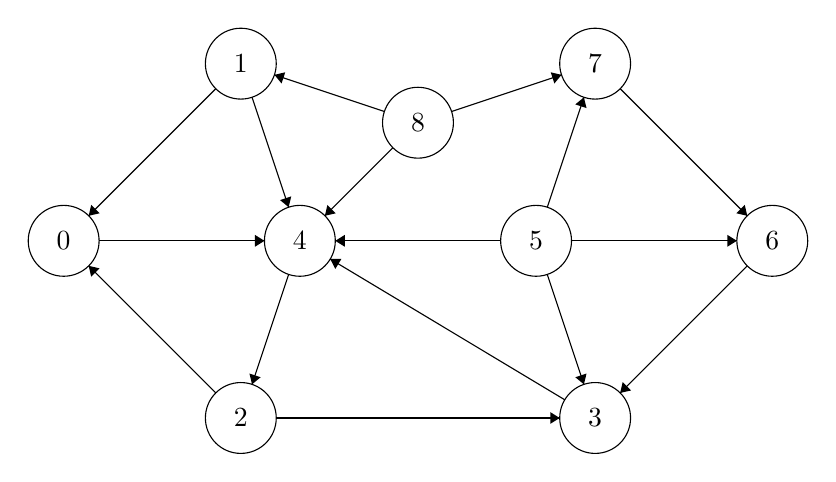
\begin{tikzpicture}[scale=0.15]
\tikzstyle{every node}+=[inner sep=0pt]
\draw (25,-15) circle (3);
\draw (25,-15) node {$1$};
\draw (10,-30) circle (3);
\draw (10,-30) node {$0$};
\draw (30,-30) circle (3);
\draw (30,-30) node {$4$};
\draw (40,-20) circle (3);
\draw (40,-20) node {$8$};
\draw (25,-45) circle (3);
\draw (25,-45) node {$2$};
\draw (55,-45) circle (3);
\draw (55,-45) node {$3$};
\draw (50,-30) circle (3);
\draw (50,-30) node {$5$};
\draw (55,-15) circle (3);
\draw (55,-15) node {$7$};
\draw (70,-30) circle (3);
\draw (70,-30) node {$6$};
\draw (22.88,-17.12) -- (12.12,-27.88);
\fill (12.12,-27.88) -- (13.04,-27.67) -- (12.33,-26.96);
\draw (25.95,-17.85) -- (29.05,-27.15);
\fill (29.05,-27.15) -- (29.27,-26.24) -- (28.32,-26.55);
\draw (37.15,-19.05) -- (27.85,-15.95);
\fill (27.85,-15.95) -- (28.45,-16.68) -- (28.76,-15.73);
\draw (37.88,-22.12) -- (32.12,-27.88);
\fill (32.12,-27.88) -- (33.04,-27.67) -- (32.33,-26.96);
\draw (13,-30) -- (27,-30);
\fill (27,-30) -- (26.2,-29.5) -- (26.2,-30.5);
\draw (22.88,-42.88) -- (12.12,-32.12);
\fill (12.12,-32.12) -- (12.33,-33.04) -- (13.04,-32.33);
\draw (29.05,-32.85) -- (25.95,-42.15);
\fill (25.95,-42.15) -- (26.68,-41.55) -- (25.73,-41.24);
\draw (28,-45) -- (52,-45);
\fill (52,-45) -- (51.2,-44.5) -- (51.2,-45.5);
\draw (52.43,-43.46) -- (32.57,-31.54);
\fill (32.57,-31.54) -- (33,-32.38) -- (33.52,-31.53);
\draw (50.95,-32.85) -- (54.05,-42.15);
\fill (54.05,-42.15) -- (54.27,-41.24) -- (53.32,-41.55);
\draw (47,-30) -- (33,-30);
\fill (33,-30) -- (33.8,-30.5) -- (33.8,-29.5);
\draw (50.95,-27.15) -- (54.05,-17.85);
\fill (54.05,-17.85) -- (53.32,-18.45) -- (54.27,-18.76);
\draw (42.85,-19.05) -- (52.15,-15.95);
\fill (52.15,-15.95) -- (51.24,-15.73) -- (51.55,-16.68);
\draw (57.12,-17.12) -- (67.88,-27.88);
\fill (67.88,-27.88) -- (67.67,-26.96) -- (66.96,-27.67);
\draw (53,-30) -- (67,-30);
\fill (67,-30) -- (66.2,-29.5) -- (66.2,-30.5);
\draw (67.88,-32.12) -- (57.12,-42.88);
\fill (57.12,-42.88) -- (58.04,-42.67) -- (57.33,-41.96);
\end{tikzpicture}
\end{center}

\begin{parts}
\part Give the depth-first \textit{pre-order} traversal of the graph.
\begin{solution}[0.5in]
\begin{verbatim}
0, 4, 2, 3, 1, 5, 6, 7, 8
\end{verbatim}
\end{solution}

\part Give the depth-first \textit{post-order} traversal of the graph.
\begin{solution}[0.5in]
\begin{verbatim}
3, 2, 4, 0, 1, 6, 7, 5, 8
\end{verbatim}
\end{solution}

\part Give the reverse depth-first \textit{post-order} traversal.
\begin{solution}[0.5in]
\begin{verbatim}
8, 5, 7, 6, 1, 0, 4, 2, 3
\end{verbatim}
\end{solution}
\end{parts}